\documentclass[../thesis/thesis.tex]{subfiles}
\begin{document}
 \chapter{Design and Implementation}
 \label{chap:design}

With the Literature Review concluding that a design based on Thermosense would be most appropriate, a software and hardware prototype (the ``sensing system'') must now be constructed to provide a platform for experimentation and evaluation of the sensor, as well as to capture, store, visualize and replay sensor data for those purposes. We will first discuss the hardware foundations of the project, then the architecture of the software developed to run on those foundations.

\section{Hardware}

As reliability and future extensibility are core concerns of the project, a three-tiered system is employed with regards to the hardware involved in the system (\Fref{tab:sensor:tiers}). At the bottom, the Sensing Tier, we have the raw sensor. Connected to the sensors via those respective protocols is the Preprocessing Tier, run an embedded system. The embedded device polls the data from these sensors, performs necessary calculations to turn raw information into suitable data, and communicates this via Serial over USB to the third tier. The third tier, the Analysis Tier, is run on a fully fledged computer. In our prototype, it captures and stores both video data, and the Temperature and Motion data it receives over Serial over USB.

While at a glance this system may seem overly complicated, it ensures that a sensible upgrade path to a more feature-rich sensing system is available. In the current prototype, the Analysis Tier merely stores captured data for offline analysis, in future prototypes this analysis can be done live and served to interested parties over a RESTful API. In the current prototype, the Analysis and Sensing Tiers are connected by Serial over USB, in future prototypes, this can be replaced by a wireless mesh network, with many Preprocessing/Sensing Tier nodes communicating with one Analysis Tier node.

\subsection{Sensing}
As discussed in the Literature Review, using an \iar appear to be the most viable way to achieve the high-level goals of this project. Thermosense \cite{beltran2013thermosense}, the primary occupancy sensor in the \iar space, used the low-cost Panasonic \geye sensor for this task. This sensor, costing around \$50, appears to be a prime candidate for use in this project, as it satisfied low-cost criteria, as well as being proven by Thermosense to be effective in this space. However, while still available for sale in the United States, we were unable to order the sensor for shipping to Australia due to export restrictions outside of our control. While such restrictions would be circumventable with sufficient effort, using a sensor with such restrictions in place goes against an implicit criteria of the parts used in the project being relatively easy to acquire.

This forced us to search for alternative sensors in the space that fulfill similar criteria but were more broadly available. The sensor we settled on was the \mlx \cite{MLXDatasheet}, an \iar with similar overall qualities that differed in several important ways; it provides a $16 \times 4$ grid of thermal information, it has an overall narrower field of view and it sells for approximately \$80. Like the \geye, the \mlx sensor communicates over the 2-wire \iic bus, a low-level bi-directional communication bus widely used and supported in embedded systems.

In an idealized version of this occupancy system, much like Thermosense this system would include wireless networking and a very small form factor. However, due to time and resource constraints, the scope of this project has been limited to a minimum viable implementation. This prototype architecture has been designed such that a clear path to an idea system architecture involving each Pre-Processing Tier and Analysis Tier being connected by a wireless mesh network to enable easy installation in households.

\begin{table}
\centering
\begin{tabular}{|r|l|}
\hline
\textbf{Analysis Tier} & Raspberry Pi B+ \\ \hline
\textbf{Preprocessing Tier} & \ard Uno R3 \\ \hline
\textbf{Sensing Tier} & \acl{mlx} \& PIR \\ \hline
\end{tabular}
\caption{Hardware tiers}
\label{tab:sensor:tiers}
\end{table}


\begin{figure}
\centering
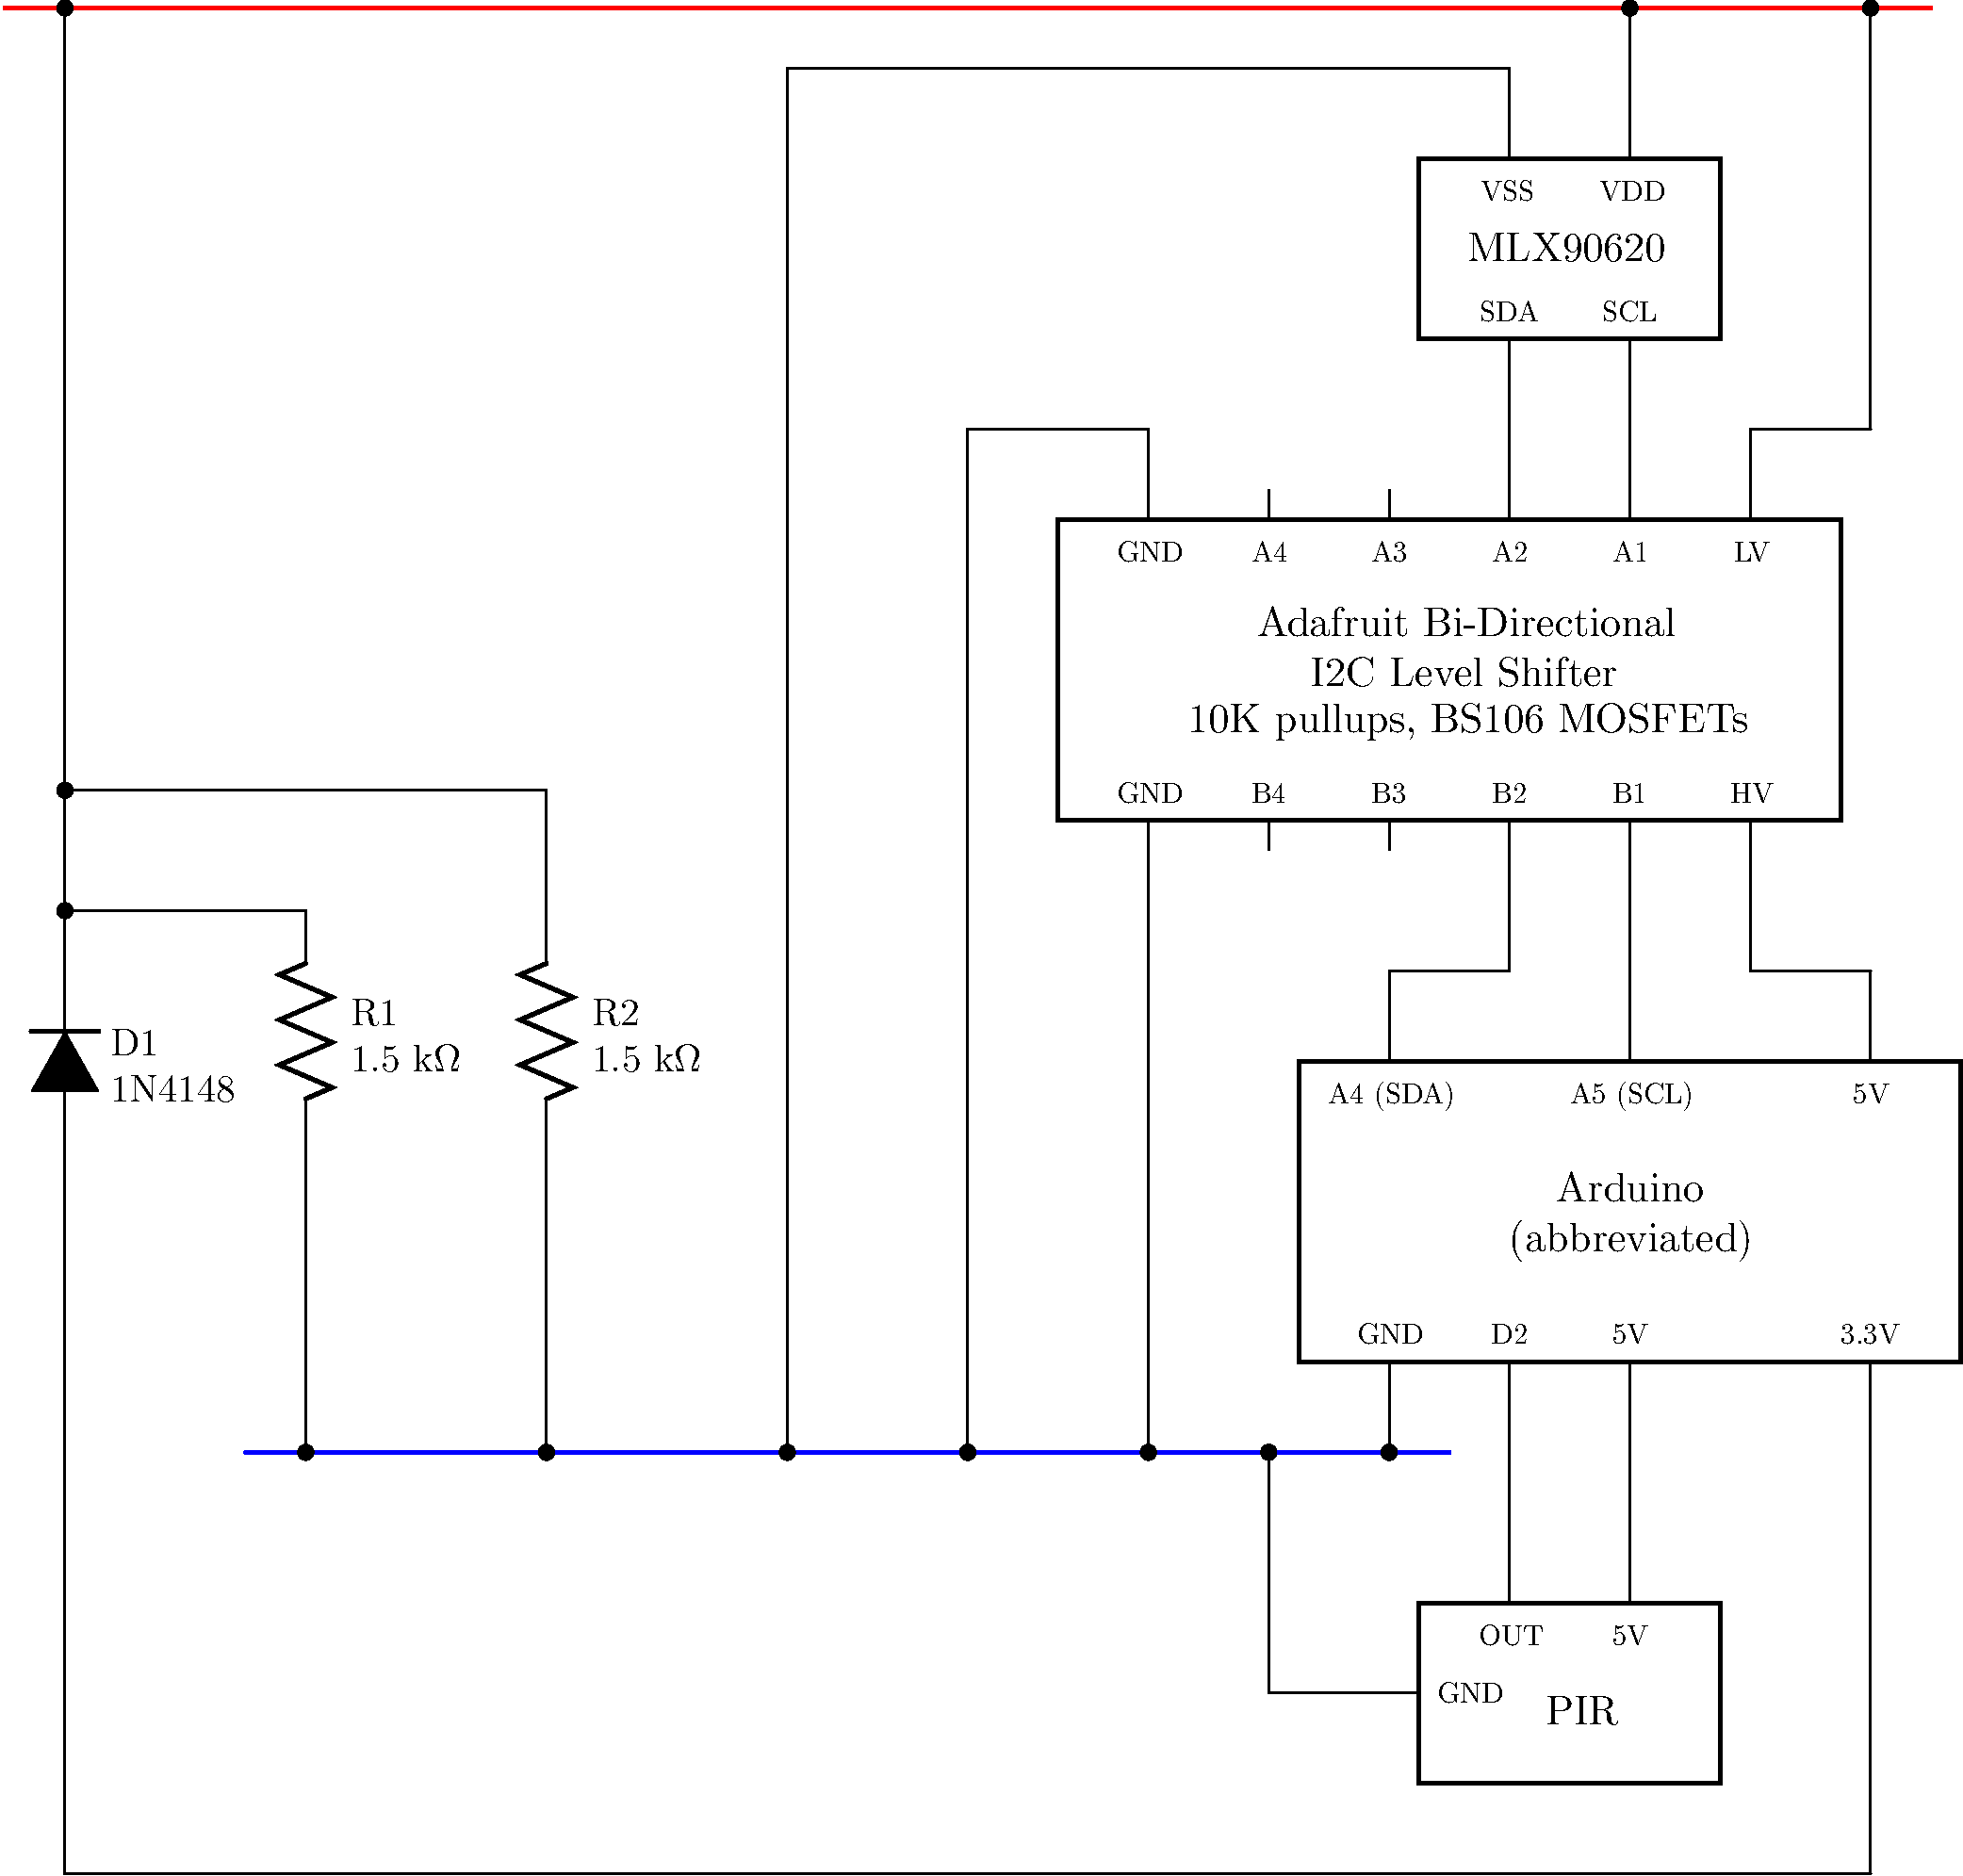
\includegraphics[width=\textwidth]{../diagrams/mlx-arduino2.pdf}
\caption{MLX90620, PIR and Arduino integration circuit}
\label{fig:circuits:node}
\end{figure}

\subsection{Pre-Processing}

Due to low cost and ease of use, the \ard platform was selected as the host for the Preprocessing Tier, and thus the low-level \iic interface for communication to the \mlx. Initially, this presented some challenges, as the \mlx recommends a power and communication voltage of 2.6V, while the \ard is only able to output 3.3V and 5V as power, and 5V as communication. Due to this, it was not possible to directly connect the \ard to the \mlx, and similarly due to the two-way nature of the \iic 2-wire communication protocol, it was also not possible to simply lower the \ard voltage using simple electrical techniques, as such techniques would interfere with two-way communication.

A solution was found in the form of a \iic level-shifter, the Adafruit ``4-channel I2C-safe Bi-directional Logic Level Converter'' \cite{AdafruitI2C}, which provided a cheap method to bi-directionally communicate between the two devices at their own preferred voltages. The layout of the circuit necessary to link the \ard and the \mlx using this converter can be seen in \Fref{fig:circuits:node}.

% TODO: Check PIR settings
Additionally, as used in the Thermosense paper, a \pir motion sensor \cite{AdafruitPIR} was also connected to the \ard. This sensor, operating at 5V natively, did not require any complex circuitry to interface with the \ard. It is connected to digital pin 2 on the \ard, where it provides a rising signal in the event that motion is detected, which can be configured to cause an interrupt on the \ard. In the configuration used in this project, the sensor's sensitivity was set to the highest value and the timeout for re-triggering was set to the lowest value (approximately 2.5 seconds). Additionally, the continuous re-triggering feature (whereby the sensor produces continuous rising and falling signals for the duration of motion) was disabled using the provided jumpers. 

\subsection{Analysis / Classification}
% Talk about RPi and prototype board, and prototype iterations

For the Analysis Tier, the Raspberry Pi B+ was chosen, as it is a powerful computer capable of running Linux available for an extraordinarily low price. The \ard is connected to the Raspberry Pi over USB, which provides it both power and the capacity to transfer data. In turn, the Raspberry Pi is connected to a simple micro-USB rechargeable battery pack, which provides it with power, and subsequently the \ard and sensors.

\subsection{Component Costs}
\label{subsec:cost}
As being low-cost is one of the project's goals, we have summarized the cost of each of the components of the prototype in \Fref{tab:sensor:cost}. We believe that for a prototype, this cost is sufficiently low. In the envisioned system, there would only be one Raspberry Pi in the system, and it would not require a camera, lowering the cost to around $\$40 + \$115n$ where $n$ is the number of sensors. Similarly, as technology improves (as discussed in later chapters), sensor technology will continue to become cheaper, causing the most expensive component, the \mlx, to lower in cost.

When we compare this to the estimated cost of the Thermosense system (\Fref{tab:sensor:thermosensecost}), we believe that it achieves a suitably comparable cost for a prototype. When removing the aspects of the prototype that would be unnecessary in the final version, the difference is less than \$15.

\begin{table}
\centering
\begin{subtable}[b]{0.5\textwidth}
\centering
\begin{tabular}{|l|r|}
\hline
\textbf{Part} & \textbf{Cost} \\ \hline
MLX90620 & \$80 \\ \hline
Raspberry Pi B+ &  \$50 \\ \hline
Arduino Uno R3 & \$40 \\ \hline
Passive Infrared Sensor & \$10 \\ \hline
\textbf{TOTAL} & \textbf{\$180} \\ \hline
\end{tabular}
\caption{Our project}
\label{tab:sensor:cost}
\end{subtable}%
~%
\begin{subtable}[b]{0.5\textwidth}
\centering
\begin{tabular}{|l|r|}
\hline
\textbf{Part} & \textbf{Cost} \\ \hline
TMote Sky & \$110 \\ \hline
Grid-EYE & \$50 \\ \hline
Passive Infrared Sensor & \$10 \\ \hline
 & \\ \hline
\textbf{TOTAL} & \textbf{\$170} \\ \hline
\end{tabular}
\caption{Thermosense (estimated)}
\label{tab:sensor:thermosensecost}
\end{subtable}
\caption{Component cost comparison}
\end{table}


\section{Software}

\begin{table}
\centering
\begin{subtable}[b]{0.5\textwidth}
\centering
\begin{tabular}{|l|r|}
\hline
\textbf{Category} & \textbf{SLOC}  \\ \hline
TArL Python       & 674            \\ \hline
\hspace{5mm}\texttt{cam}        & 425           \\ \hline
\hspace{5mm}\texttt{features}   & 191           \\ \hline
\hspace{5mm}\texttt{pxdisplay}  & 58            \\ \hline
TArL Arduino  & 492            \\ \hline
\hspace{5mm}\texttt{mlx90620\_driver}  & 492          \\ \hline
Analysis Scripts  & 147            \\ \hline
Capture Scripts   & 234            \\ \hline
\textit{Total}    & \textit{1,624} \\ \hline
\end{tabular}
\caption{Source Lines Of Code written}
\end{subtable}%
~%
\begin{subtable}[b]{0.5\textwidth}
\centering
\begin{tabular}{|l|l|}
\hline
\textbf{Library}     & \multicolumn{1}{l|}{\textbf{Version}} \\ \hline
\multicolumn{2}{|c|}{Arduino}                                \\ \hline
SDK                  & 1.6.4                                 \\ \hline
\texttt{SimpleTimer} & 1.0                                   \\ \hline
\multicolumn{2}{|c|}{Python}                                 \\ \hline
\texttt{networkx}    & 1.9.1                                 \\ \hline
\texttt{numpy}       & 1.8.0                                 \\ \hline
\texttt{matplotlib}  & 1.3.1                                 \\ \hline
\texttt{picamera}    & 1.10                                  \\ \hline
\texttt{Pillow}      & 2.8.1                                 \\ \hline
\end{tabular}
\caption{Libraries used}
\end{subtable}
\caption{Overview of code used in project}
\end{table}

At each layer of the described three-tier software architecture (pictured in greater detail in \Fref{fig:pictures:protob-arch}), there must exist software which governs the operation of that tier's processing concerns. A bi-lingual software library, the Thermal Array Library (TArL), was developed to provide a suite of functions to enable the easy data collection and analysis of information from the hardware prototype.

\begin{figure}
\centering
\begin{tikzpicture}[node distance=1.7cm]
\node (interwebs) [cbox] {Network};
\node (wifi) [dashbox, right=of interwebs] {\small WiFi / Ethernet};
\node (rpi) [fcont, below=of wifi] {Raspberry Pi B+ \linebreak
  ``Analysis Tier'' \linebreak
 
  \tikz\node[fbox] {\small TArL Python Library};
};
\node (cam) [box, right=of rpi] {Camera};
\node (usb) [dashbox, below=of rpi] {\small Serial over USB};
\node (ard) [fcont, below=of usb] {Arduino Uno R3 \linebreak
  ``Preprocessing Tier'' \linebreak
  
  \tikz\node[fbox] {\small TArL C++ Driver};
};
\node (iic) [dashbox, left=of ard] {\small \iic};
\node (mlx) [box, below=of iic] {MLX90620};
\node (wire) [dashbox, right=of ard] {\small Interrupt};
\node (pir) [box, below=of wire] {PIR};
\node (sensetier) [dashbox, dotted, fit=(pir) (mlx)] {``Sensing Tier''};

\draw [line] (interwebs) -- (wifi);
\draw [line] (wifi) -- (rpi);
\draw [line] (rpi) -- (usb);
\draw [line] (usb) -- (ard);
\draw [line] (ard) -- (iic);
\draw [line] (iic) -- (mlx);
\draw [line] (ard) -- (wire);
\draw [line] (wire) -- (pir);
\draw [line] (rpi) -- (cam);
\end{tikzpicture}
\caption{Prototype system architecture}
\label{fig:pictures:protob-arch}
\end{figure}

At the Sensing Tier, it was not necessary for any software to be developed, as any software necessary came pre-installed and ready for use on the aforementioned sensors.

At the Preprocessing Tier, the Arduino, the default C++ derivative language was used, as careful management of memory usage and algorithmic complexity is required in such a resource-constrained environment, thus limiting choice in the area.

Finally, at Analysis Tier, a computer running fully-fledged Linux, choice of language becomes a possibility. In this instance, Python was settled on as the language of choice, as it is a quite high-level language with excellent library support for the functions required of the Analysis Tier, including serial interface, the use of the Raspberry Pi's built in camera, and image analysis. The 2.x branch of Python was chosen over the 3.x branch, despite its age, due a greater maturity in support for several key graphical interface libraries.

\subsection{Sensing}
The \mlx itself is its own computer (see \Fref{fig:exps:blockdia}), containing EEPROM storage, RAM and unspecified code to perform ``digital filtering'' on the $16 \times 4$ array of digital active thermopiles. We are able to communicate with the \mlx through the provided \iic interface, which offers commands to read both the EEPROM, and the sensor's RAM directly. 

The sensor's EEPROM contains configuration values that the interfacing device is required to input into the device's RAM as part of a multi-step initialization sequence, and also contains constants used as part of the raw data to \dc conversion process. The sensor's RAM contains the post-filtered but still very raw thermopile values, which are updated with reference to a clock frequency set between 0.5Hz to 512Hz in the initialization process.

The sensor's documentation offers no information regarding reconfiguration of the sensor's internal programming code, nor what code exists on the sensor when purchased. As such, we refer to the sensor's dataset \cite{MLXDatasheet} and use only the specified commands to interface with the sensor, and later on will perform experiments to determine the properties of the sensor.

\begin{figure}
\centering
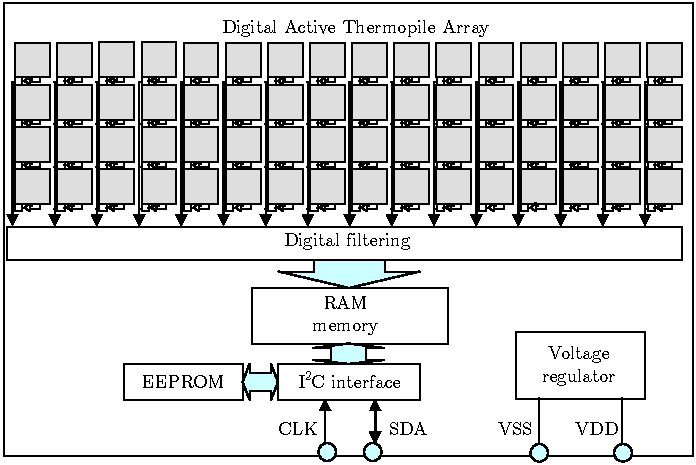
\includegraphics[width=0.8\textwidth]{../diagrams/mlx-block-diagram.pdf}
\caption{Block diagram for the \mlx taken from datasheet \cite{MLXDatasheet}}
\label{fig:exps:blockdia}
\end{figure}

\subsection{Pre-Processing}

On the Arduino, once large program was developed, termed \texttt{mlx90620\_driver.ino}. This program's purpose was to take simple commands over serial to configure the \mlx and to report back the current temperature values and \pir motion information at either a pre-set interval, or when requested.

To calculate the final temperature values that the \mlx offers, a complex initialization and computational process must be followed, which is specified in the sensor's datasheet \cite{MLXDatasheet}. This process involves initializing the sensor with values attained from a separate on-board \iic EEPROM, then retrieving a variety of normalization and adjustment values, along with the raw sensor data, to compute the final temperature result.

The basic algorithm to perform this normalization was based upon the provided datasheet \cite{MLXDatasheet}, as well as code by users ``maxbot'', ``IIBaboomba'', ``nseidle'' and others on the Arduino Forums \cite{ArduinoForum} and was modified to operate with the newer \ard ``Wire'' \iic libraries released since the authors' posts. In pursuit of the project's aims to create a more approachable thermal sensor, the code was also restructured and rewritten to be both more readable, and to introduce a set of features to make the management of the sensor data easier for the user, and for the information to be more human readable.

Additionally, support for the \pir's motion data was added to the code, with the \pir configured to perform interrupts on one of the Arduino's digital pin and the code structured to take note of this information and to report it to the user in the ``MOTION'' section of the next packet.

The first of the features introduced was the human-readable format for serial transmission. This allows the user to both easily write code that can parse the serial to acquire the serial data, as well as examine the serial data directly with ease. When the \ard first boots running the software, \Fref{fig:code:initseq} is output. This specifies several things that are useful to the user; the attached sensor (``DRIVER''), the build of the software (``BUILD'') and the refresh rate of the sensor (``IRHZ''). Several different headers, such as ``ACTIVE'' and ``INIT'' specify the current millisecond time of the processor, thus indicating how long the execution of the initialization process took (33 milliseconds).

Once booted, the user is able to send several one-character commands to the sensor to configure operation, which are described in \Fref{tab:ardcommands}. Depending on the sensor configuration, IR data may be periodically output automatically, or otherwise manually triggered. This IR data is produced in the packet format described in \Fref{fig:code:initseq}. This is a simple, human readable format that includes the millisecond time of the processor at the start and end of the calculation, if the \pir has seen any motion for the duration of the calculation, and the 16x4 grid of calculated temperature values.

\begin{figure}
 \centering
\begin{minted}[frame=single,fontsize=\scriptsize]{text}
INIT 0
INFO START
DRIVER MLX90620
BUILD Feb  1 2015 00:00:00
IRHZ 1
INFO STOP
ACTIVE 33

START 34
MOVEMENT 0
1.0  1.0  1.0  1.0  1.0  1.0  1.0  1.0  1.0  1.0  1.0  1.0  1.0  1.0  1.0  1.0
1.0  1.0  1.0  1.0  1.0  1.0  1.0  1.0  1.0  1.0  1.0  1.0  1.0  1.0  1.0  1.0
1.0  1.0  1.0  1.0  1.0  1.0  1.0  1.0  1.0  1.0  1.0  1.0  1.0  1.0  1.0  1.0
1.0  1.0  1.0  1.0  1.0  1.0  1.0  1.0  1.0  1.0  1.0  1.0  1.0  1.0  1.0  1.0
STOP 97
\end{minted}
%\begin{tabular}{|l|l|}
%\hline
%\texttt{R} & Flush buffers and reset \ard \\ \hline
%\texttt{I} & Print INFO again \\ \hline
%\texttt{T} & Activate timers for periodic IR data output \\ \hline
%\texttt{O} & Deactivate timers for periodic IR data output \\ \hline
%\texttt{P} & Manually trigger capture and output of IR data \\ \hline
%\texttt{F\textit{x}} & Set sensor refresh frequency to \textit{x} and reboot \\ \hline
%\end{tabular}
\caption{Initialisation sequence and thermal packet}
\label{fig:code:initseq}
\end{figure}

\subsection{Analysis / Classification}

On the analysis tier, TArL's set of Python libraries and accompanying capture and analysis scripts were developed to interface with the Arduino, parse and interpret its data, and to provide data logging and visualization capabilities.

\texttt{TArL}'s Python portion provides 4 main feature sets across 3 files; the \texttt{Manager} series of classes, the \texttt{Visualizer} class, the \texttt{Features} class and the \texttt{pxdisplay} module.

\subsubsection*{\texttt{Manager} classes}
The Manager series of classes are the direct interface between the Arduino and the Python classes. They implement a multi-threaded serial data collection and parsing system which converts the raw serial output of the connected Arduino into a series of Python data structures that represent the collected temperature and motion data of each captured frame. Several different versions of the \texttt{Manager} class exist to perform slightly different functions. When initializing these classes the sample rate of the \mlx can be configured, and it will be sent through to the Arduino for updating.

\texttt{BaseManager} is responsible for the implementation of the core serial parsing functions. It also provides a threaded interface through which the \mlx's continuous stream of data can be subscribed to by other threads. The primary API, the \texttt{subscribe\_} series of functions, return a thread-safe queue structure, through which thermal packets can be received by various other threads when they become available.

\texttt{Manager}, the primary class, provides access the \mlx's data at configurable intervals. When initializing this class, you may specific 0.5, 1, 2, 4 or 8Hz, and the class will configure the Arduino to both set the \mlx to this sample rate, and to automatically write this data to the serial buffer whenever it is available. This serial interface is multi-threaded, as at higher serial baud rates if data was not polled continuously enough the internal serial buffer would fill and some data would be discarded. By ensuring this process cannot be blocked by other parts of the running program this problem is mostly eliminated. 

\texttt{OnDemandManager} operates in a similar way to \texttt{Manager}, however instead of using a non-blocking threaded approach, the user's scripts may request thermal/motion data from the class, and it will poll the Arduino for information and block until this information is parsed and returned.

Finally, \texttt{ManagerPlaybackEmulator} is a simple class which can take a previously created thermal recording from a file, and emulate the \texttt{Manager} class by providing access to thread-safe queues which return this data at the specified Hz rate. This class can be used as a means to playback thermal recordings with the same visualization functions.

\subsubsection*{\texttt{pxdisplay} functions}

The \texttt{pxdisplay} module is a set of functions that utilize the \texttt{pygame} library to create a simple live-updating window containing a thermal map representation of the thermal data. One can generate any number of \texttt{pxdisplay} objects, which leverage the \texttt{multithreading} library and \texttt{multithreading.Queue} to allow thermal data to be sent to the display.

The class also provides a set of functions to set a ``hotest'' and ``coldest'' temperature and have RGB colors assigned from red to blue for each temperature that falls between those two extremes.

\subsubsection*{\texttt{Visualizer} class}
The \texttt{Visualizer} class is the natural compliment to the \texttt{Manager} series of classes. The functions contained within can usually be provided with a Queue object (generated by a \texttt{Manager} class) and can perform a variety of visualization and storage functions.

From the recording side, the \texttt{Visualizer} class can ``record'' a thermal capture by saving the motion and thermal information to a simple \texttt{.tcap} file, which stores the sample rate, timings, thermal and motion data from a capture in a very straightforward format. The class can also read these files back into the data structures \texttt{Visualizer} uses internally to store data. If \texttt{Visualizer} is running on a Raspberry Pi, it can also leverage the \texttt{picamera} library an the \texttt{OnDemandManager} class to synchronously capture both visual and thermal data for ground truth purposes.

From the visualization side, \texttt{Visualizer} can leverage the \texttt{pxdisplay} module to create thermal maps that can update in real-time based on the thermal data provided by a \texttt{Manager} class. The class can also generate both images and movie files from thermal recordings using the PIL and ffmpeg libraries respectively.

\subsubsection*{\texttt{Features} class}

In Thermosense \cite{beltran2013thermosense}, an algorithm was demonstrated that allowed the separation of ``background'' information from ``active'' pixels, and from that information, the extraction of the features necessary for a classifier to correctly determine the number of people in an $8\times8$ thermal image. This algorithm involved calculating the average and standard deviations of each pixel while it is guaranteed that the image would be empty, and then when motion is detected, considering any pixel ``active'' that reaches a value more than 3 standard deviations above the pixel when there was no motion.

From these ``active'' pixels, it was established that a set of three feature vectors were all that were required to correctly classify the number of people in the thermal image. These feature vectors were;
\begin{enumerate}
\item \textbf{Number of active pixels}: The total number of pixels that are considered ``active'' in a given frame
\item \textbf{Number of connected components}: If each active pixel is represented as an node in an undirected graph where adjacent active pixels are connected, how many connected components does this graph have?
\item \textbf{Size of largest connected component}: The number of active pixels contained within the largest connected component
\end{enumerate}

In accordance with the pseudo-code outlined in the Thermosense paper, the algorithm described in \Fref{lst:exps:featcode} was created to extract these figures. The portion of this code dealing with scaling the thermal background for rooms without motion was not implemented, as in all experiments tested, there exists a significant interval of time during which the no motion is guarenteed and the thermal background can be generated. The \texttt{networkx} library was used to generate the connected components information.

\begin{listing}
\centering
%TC:ignore
\begin{minted}[fontsize=\footnotesize,frame=single,breaklines=true,mathescape]{python}
# INITILISATION: Import libs, set up variables
import math, itertools, networkx

w, h       = 16, 4       # Get thermal image dimensions
wgt        = 0.01        # Weighting for exp. weighted moving avg.
fst_frame  = get_frame() # 1st thermal frame, set elsewhere (2D array)
back       = fst_frame   # Thermal background $b$ (2D array)
means      = fst_frame   # Per pixel $\bar{x}$ (2D array)
pstds      = [[0]*w]*h   # Per pixel intermediate $\sigma$ (2D array of 0) 
stds       = [[0]*w]*h   # Per pixel complete $\sigma$ (2D array of 0)
n          = 1           # Processed frames counter

# f: New frame received from sensor, starting at the 2nd frame (2D array)
# is_motion: If there has been motion detected over given time window.
def get_features(f, is_motion):
  n      += 1                # Increment frame counter
  active  = []               # Init empty active list
  g       = networkx.Graph() # Init graph structure

  # BACKGROUND UPDATE: Iterate over every pixel and update if no motion
  for i, j in itertools.product( range(w), range(h) ):
    # If no motion update $b_{i,j}$, $\bar{x}_{i,j}$, & $\sigma_{i,j}$  with $f_{i,j}$  
    if not is_motion:
      back[i][j]   = wgt * f[i][j] + (1 - wgt) * back[i][j]     # $b_{i,j}$
      means[i][j]  = means[i][j] + (f[i][j] - means[i][j]) / n  # $\bar{x}_{i,j}$
      pstds[i][j]  = pstds[i][j] + (new[i][j] - means[i][j])
                       * (c - means[i][j])
      stds[i][j]   = math.sqrt(pstds[i][j] / (n-1))             # $\sigma_{i,j}$
        
    # GRAPH GENERATION: If $(f_{i,j} - b_{i,j}) > 3\sigma_{i,j}$ add pixel to active & graph
    if (f[i][j] - back[i][j]) > (3 * stds[i][j]):
      active.append((i,j))

      # Link all adjacent active pixels in graph structure
      for ix, jx in [(-1, -1), (-1, 0), (-1, 1), (0, -1)]:
        g.add_edge((i,j), (i+ix,j+jx)) if (i+ix, j+jx) in active

  # CONNECTED COMPONENTS: Get connected comps. from graph & gen features
  cons           = list( networkx.connected_components(g) )
  num_active     = len(active)
  num_connected  = len(cons)
  size_connected = max(len(c) for c in cons) if len(cons) > 0 else None

  return (num_active, num_connected, size_connected)
\end{minted}
%TC:endignore
\caption{Core feature extraction code}
\label{lst:exps:featcode}
\end{listing}

% TODO Talk about ground truth generation script

\section{Summary}
We believe that the hardware and software architecture presented here lays a solid foundation on which experimental data can be collected. The hardware architecture, as discussed, as been specifically selected to ensure that there is a transition path from the current USB Serial Pre-Processing/Analysis connection to one which does this wirelessly. The software library, TArL, has been written to be robust and general, so that its functionality is both useful in the current situation, and also for future experiments with this and other prototypes.
 
 \ifcsdef{mainfile}{}{\bibliography{../references/primary}}
\end{document}
